\documentclass[aspectratio=169]{beamer}
\usepackage[utf8]{inputenc}
\usepackage{amsmath}
\usepackage[ngerman]{babel}
\usepackage{xcolor}
\usepackage{listings}
%\usepackage[automark]{scrpage2}
\usepackage[]{graphicx, import} 
\usepackage{subfigure}
\usepackage{wrapfig}
\usepackage[scaled]{helvet}
\renewcommand*\familydefault{\sfdefault}
%\usepackage{enumitem}
\usepackage[comma]{natbib}
\usepackage{url}
\usepackage{import}
\usepackage{gensymb}
\bibliographystyle{dcu}
%\citationstyle{dcu}
%\setbeamertemplate{footline}[page number]
\usetheme{FHNW}
\usecolortheme{seagull}
\usepackage{multimedia}
\usepackage{tikz}
\usepackage{hyperref}




\begin{document}
% infos for pdf document settings
\pdfinfo{
/Author (Stefan Blaser, FHNW - IVGI)
/Title (Entwicklung des Multisensorsystems BIMAGE.CapturePro-Backpack für die kinematische bildbasierte Innenraumaufnahme)
/Subject (Besuch DGfK Südbaden)
/Keywords (Mobile Mapping, Multisensorsystem, BIM, Indoor, Python, ROS)}

% infos for title page
\title{\textbf{Entwicklung des Multisensorsystems BIMAGE.\-Capture\-Pro-Backpack für die kinematische bildbasierte Innenraumaufnahme}}
\subtitle{Besuch DGfK Südbaden}
\author{Stefan Blaser}
\institute{Institut Vermessung und Geoinformation}
\date{26. Oktober 2017}

% title page
\begin{frame}
 \titlepage
 % - evtl. Backpack-Foto
\end{frame}

% project video
\begin{frame}[plain]
  \begin{tikzpicture}[remember picture,overlay]
    \node[anchor=south west, inner sep=0pt] at (current page.south west) {
    \movie[showcontrols, autostart]{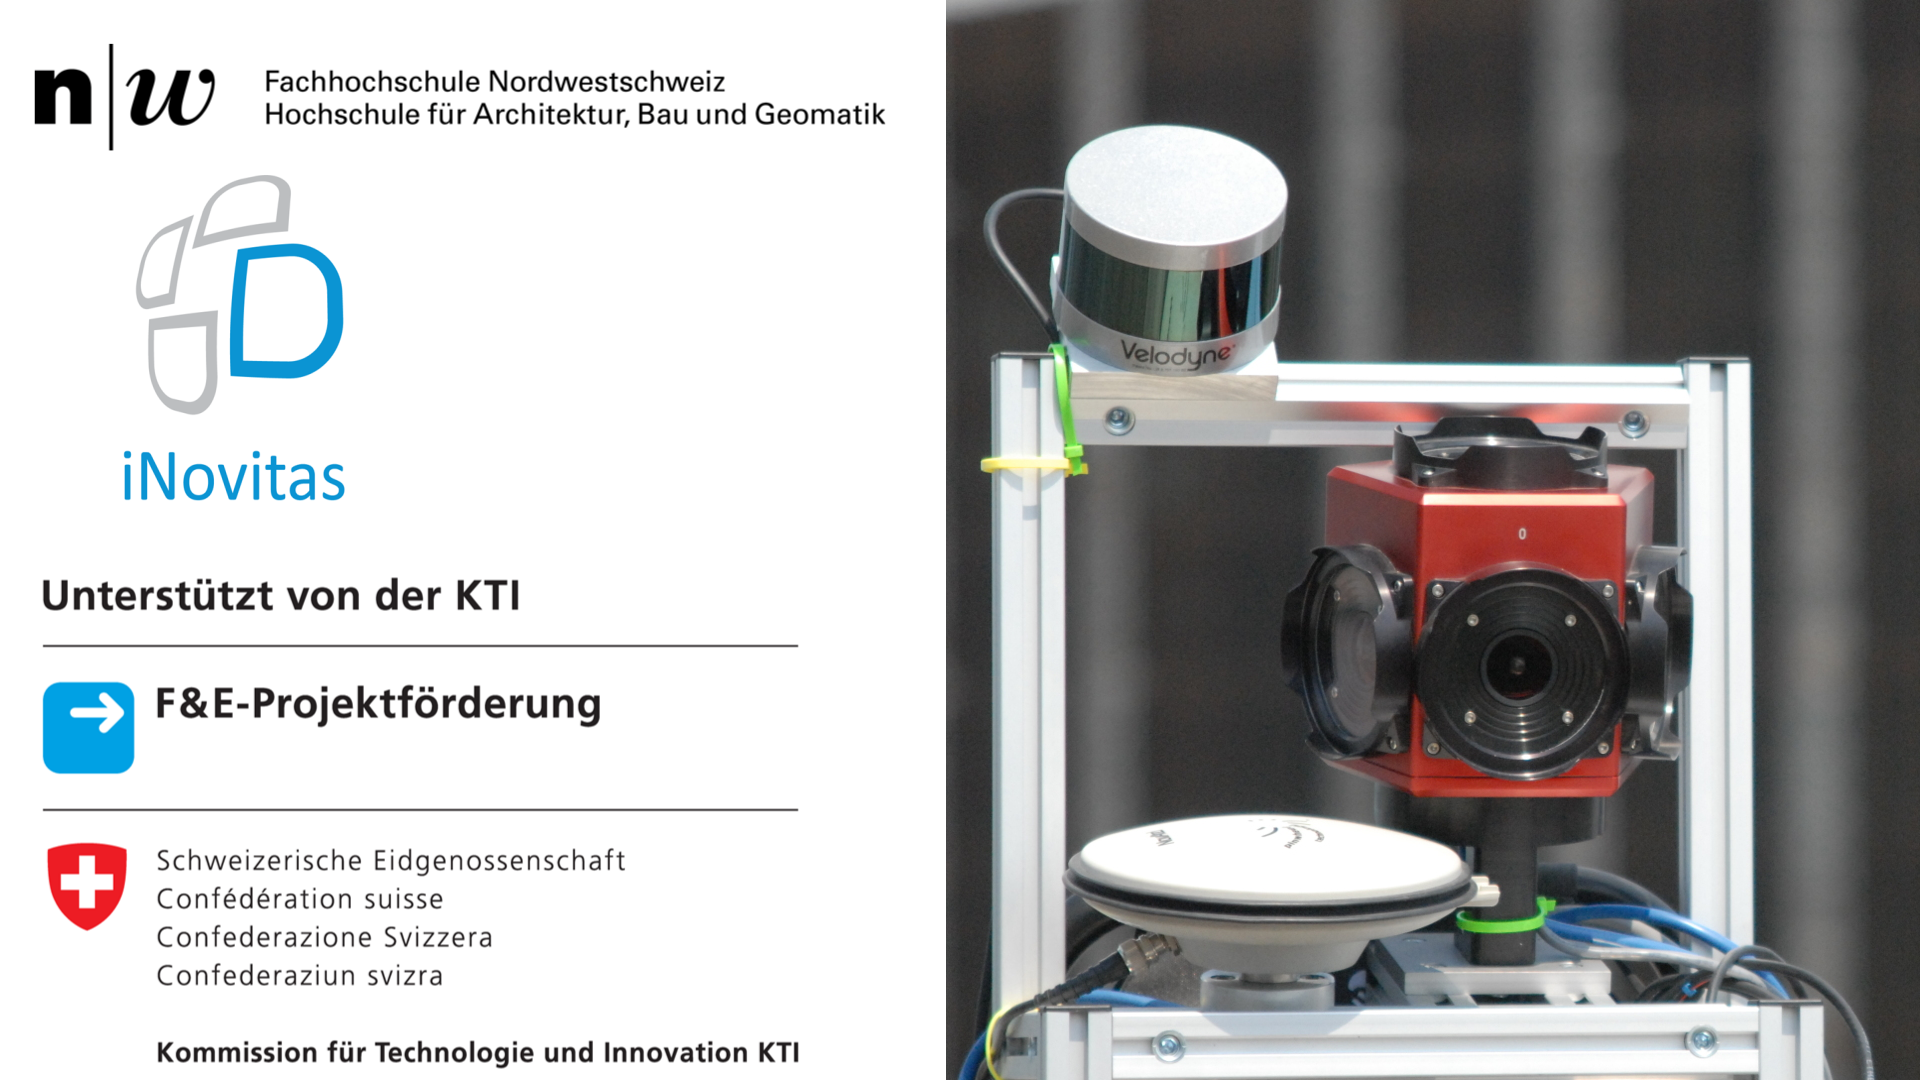
\includegraphics[width=1\paperwidth]{./Abbildungen/Projektpartner.png}}{./Abbildungen/pr_video_bimage_web.mp4}
    };
  \end{tikzpicture}
\end{frame}

% evolution
\begin{frame}
\frametitle{CapturePro -- Entwicklung}
  \begin{columns}[onlytextwidth]
    \begin{column}{0.33\textwidth}
      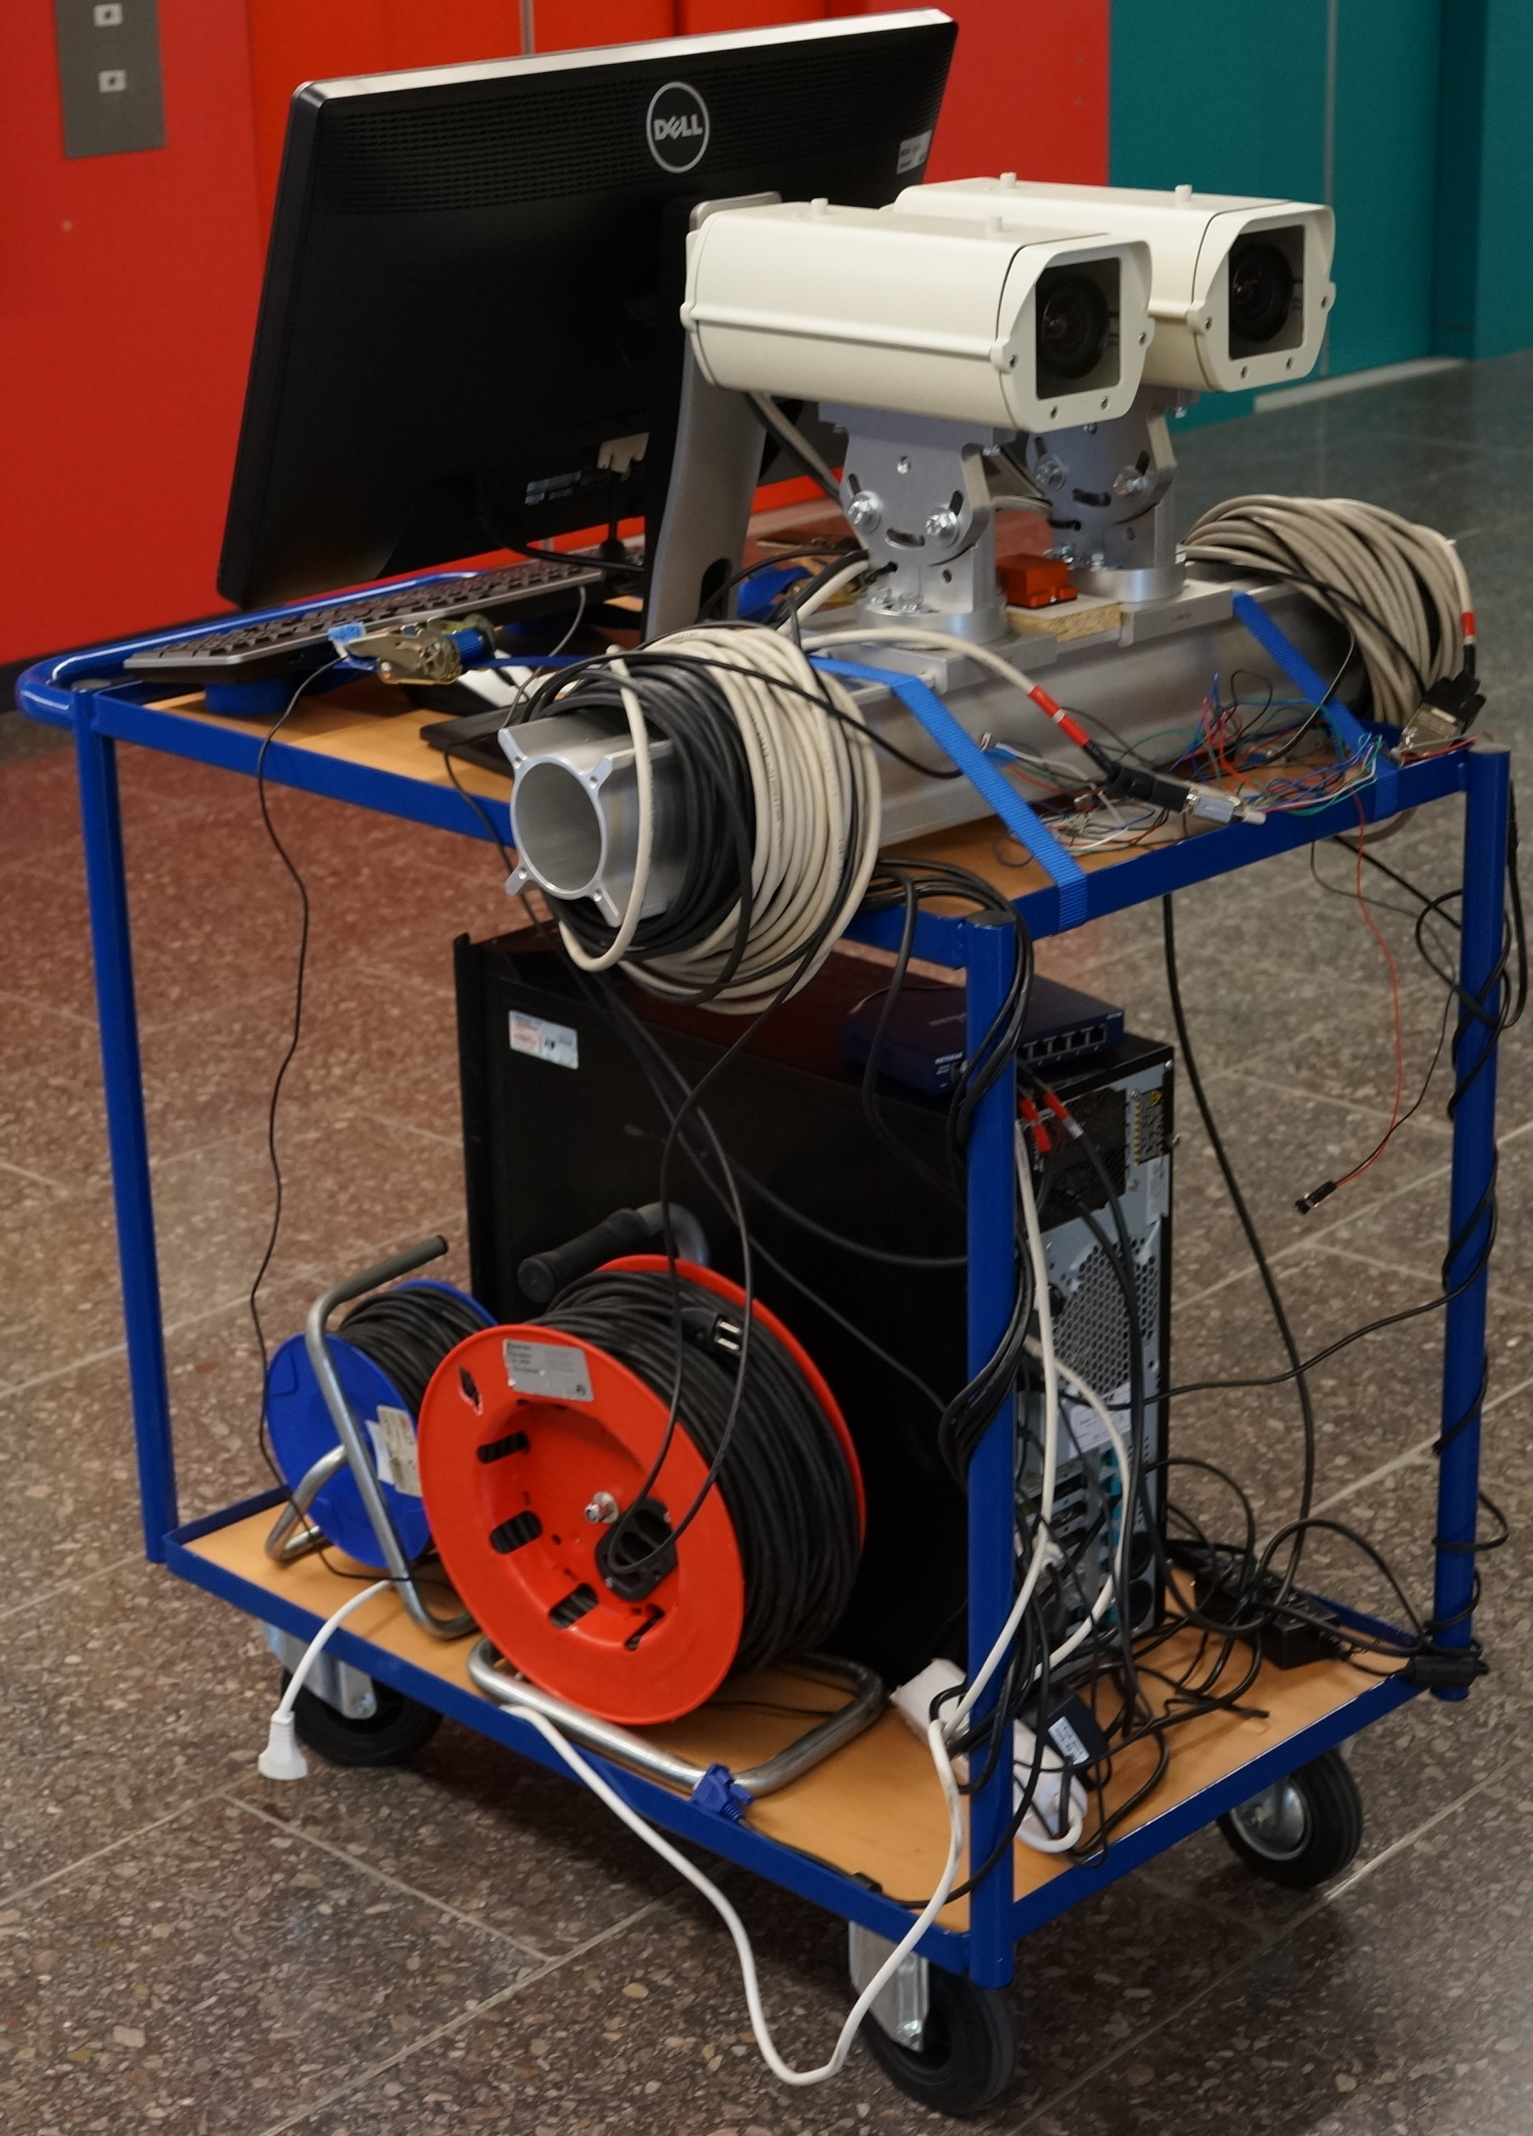
\includegraphics[height=0.7\textheight]{./Abbildungen/cappro_1.JPG}
      \\
      Sensorintegration
    \end{column}
    \begin{column}{0.33\textwidth}
      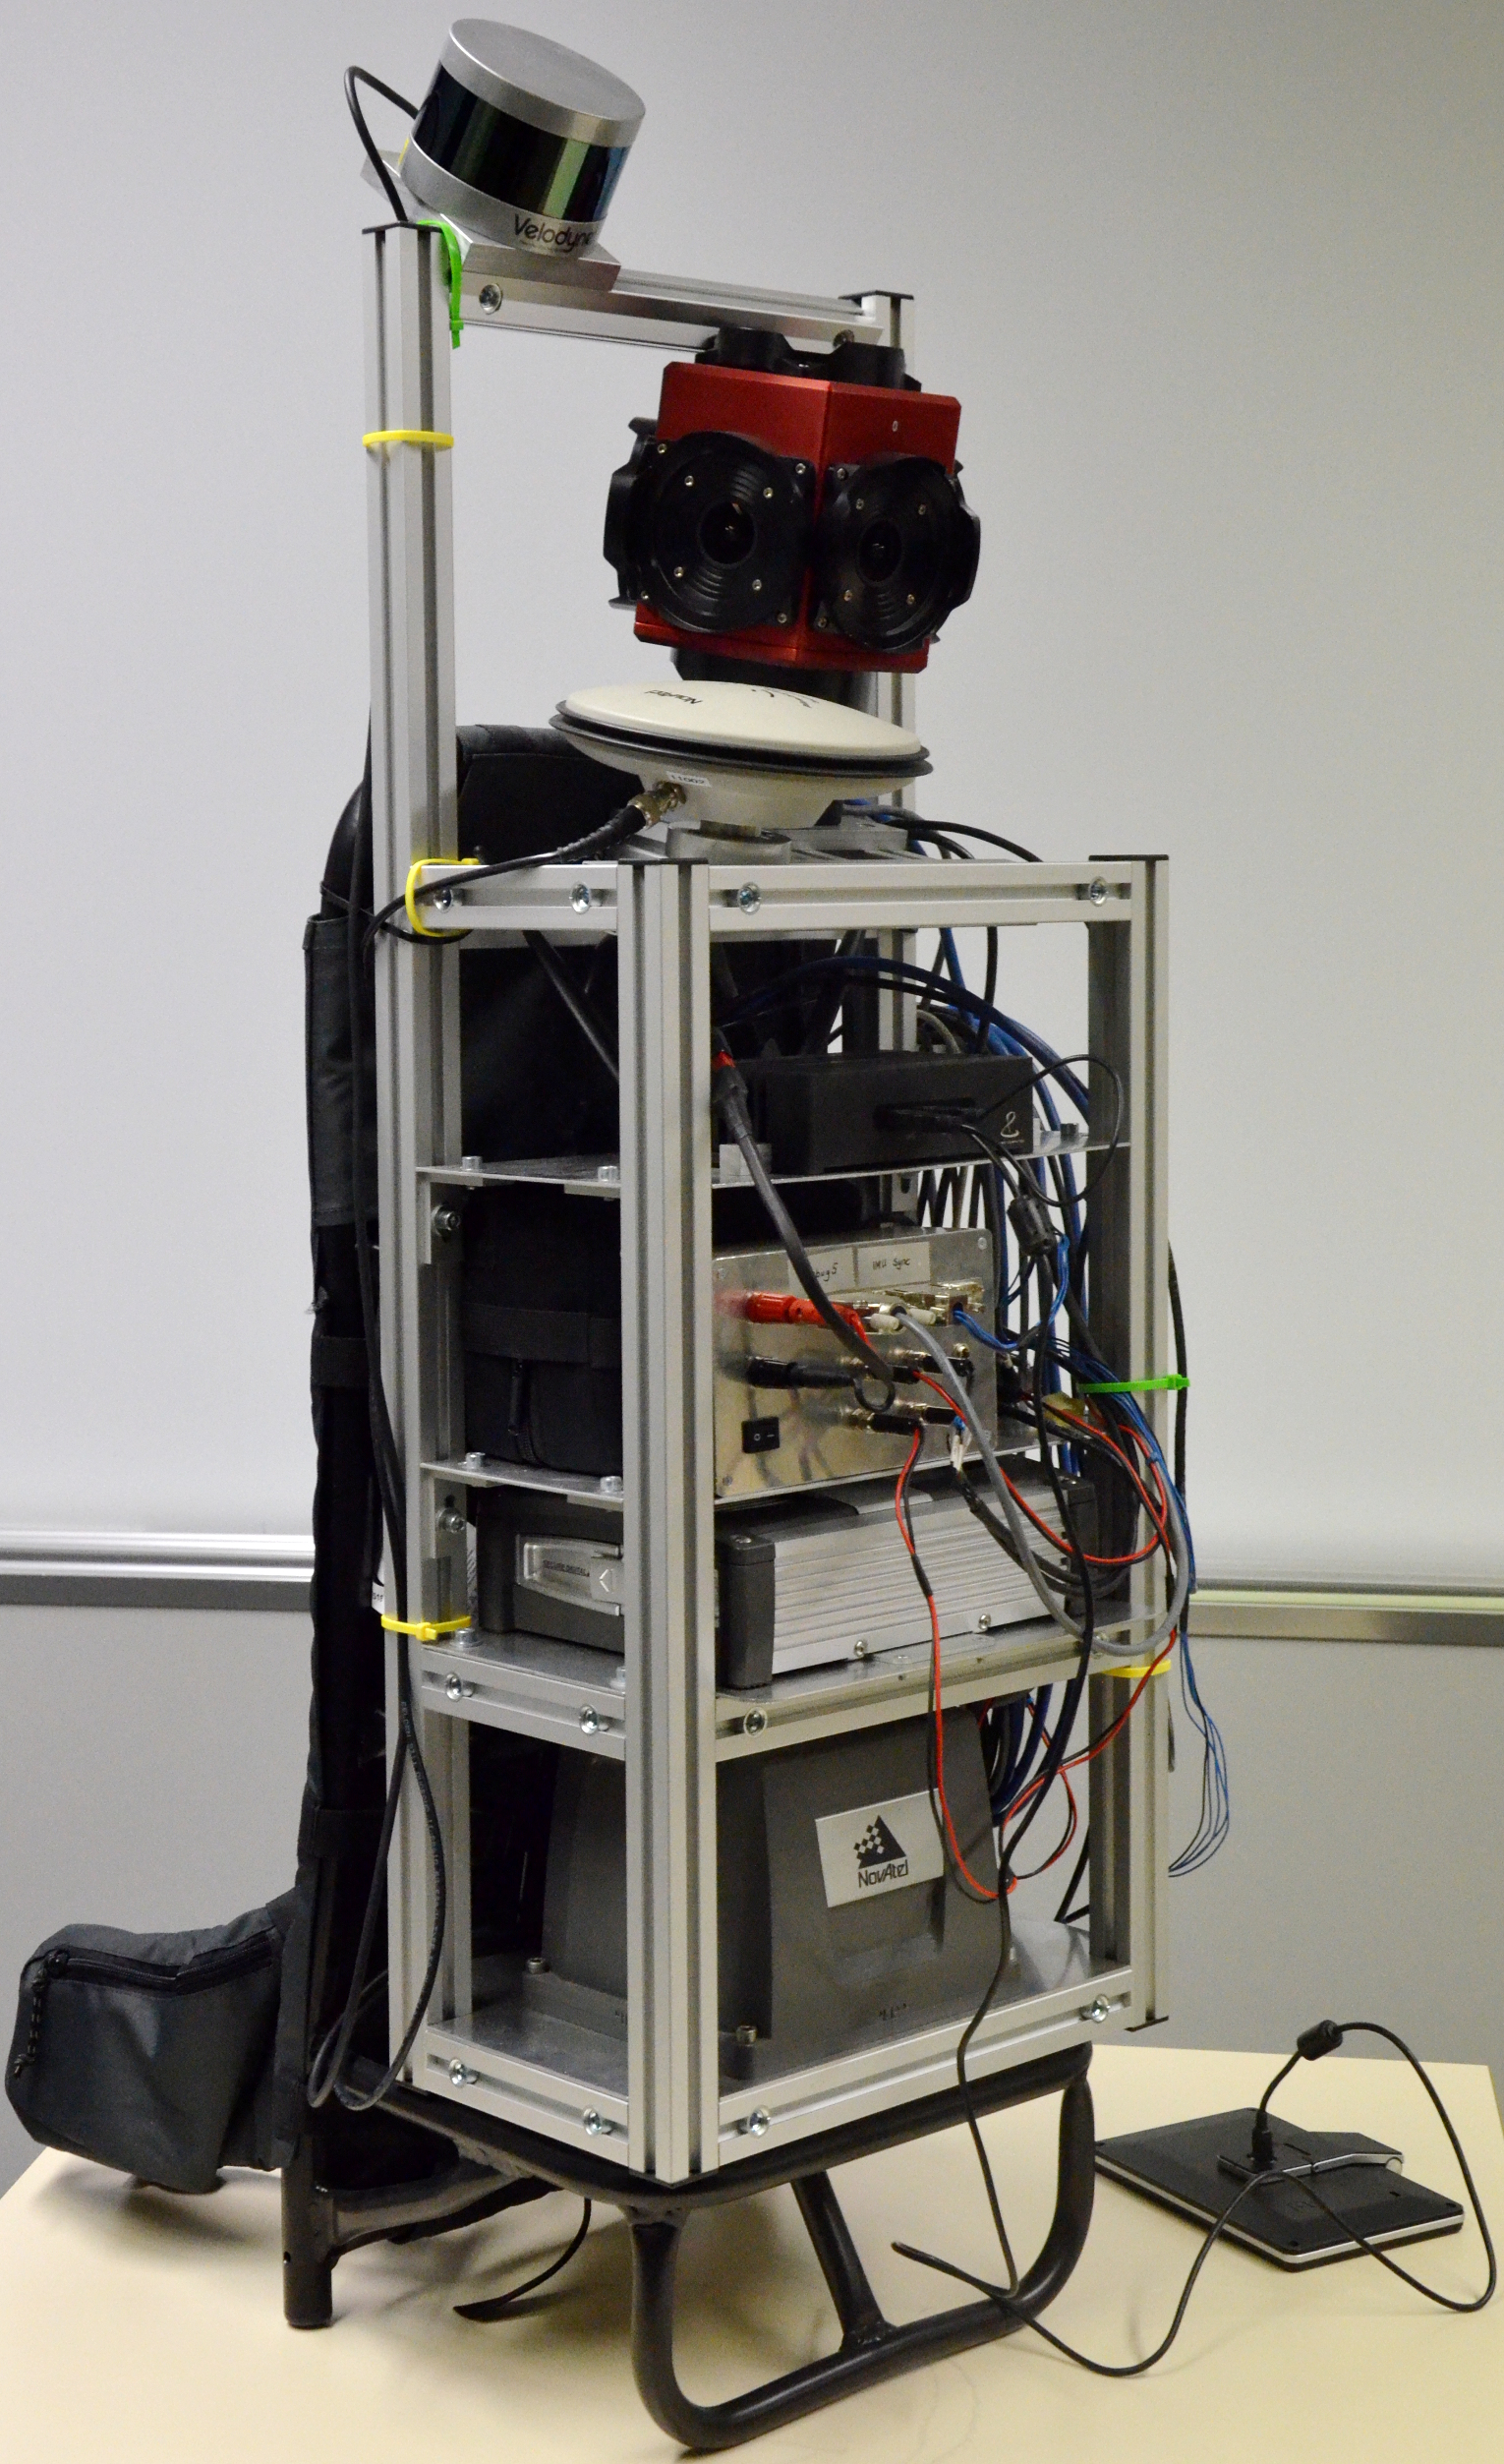
\includegraphics[height=0.7\textheight]{./Abbildungen/cappro_2.JPG}
      \\
      Datenerfassung
    \end{column}
    \begin{column}{0.33\textwidth}
      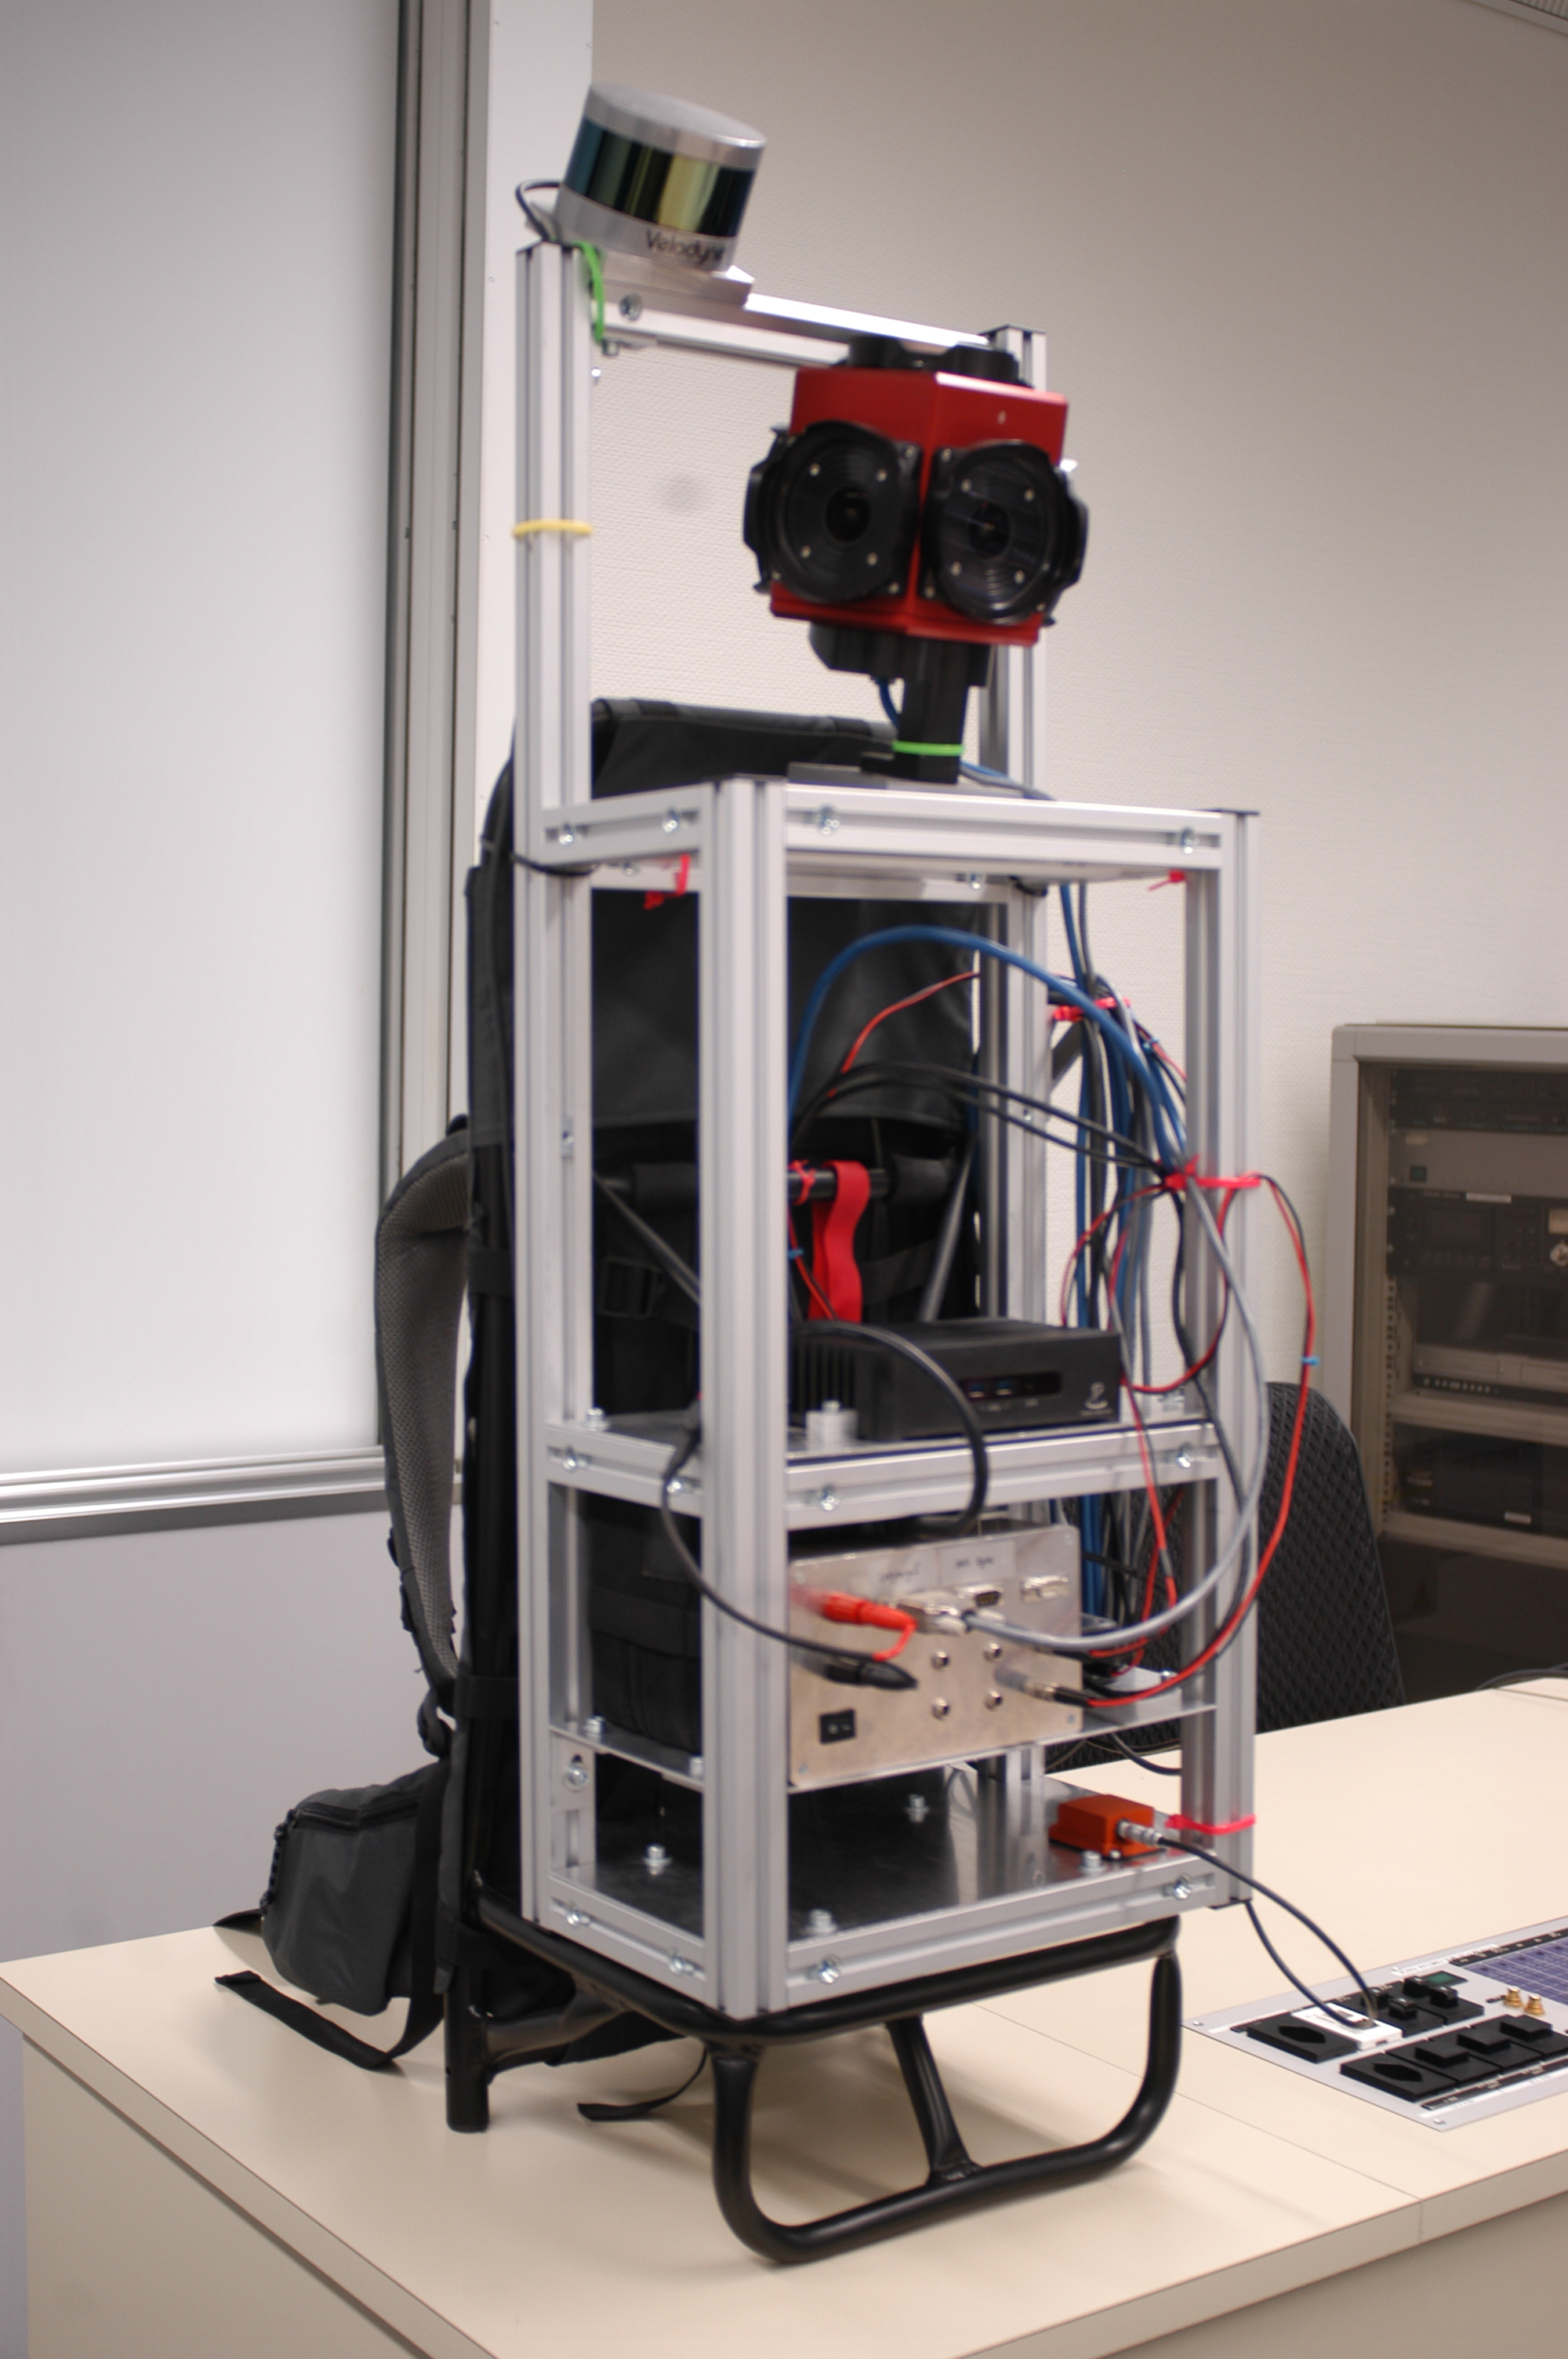
\includegraphics[height=0.7\textheight]{./Abbildungen/cappro_3.JPG}
      \\
      Online-SLAM
    \end{column}
  \end{columns}
\end{frame}

% aktueller Stand
\begin{frame}
\frametitle{Aktueller Status}
  \begin{columns}[onlytextwidth]
    \begin{column}{0.33\textwidth}
      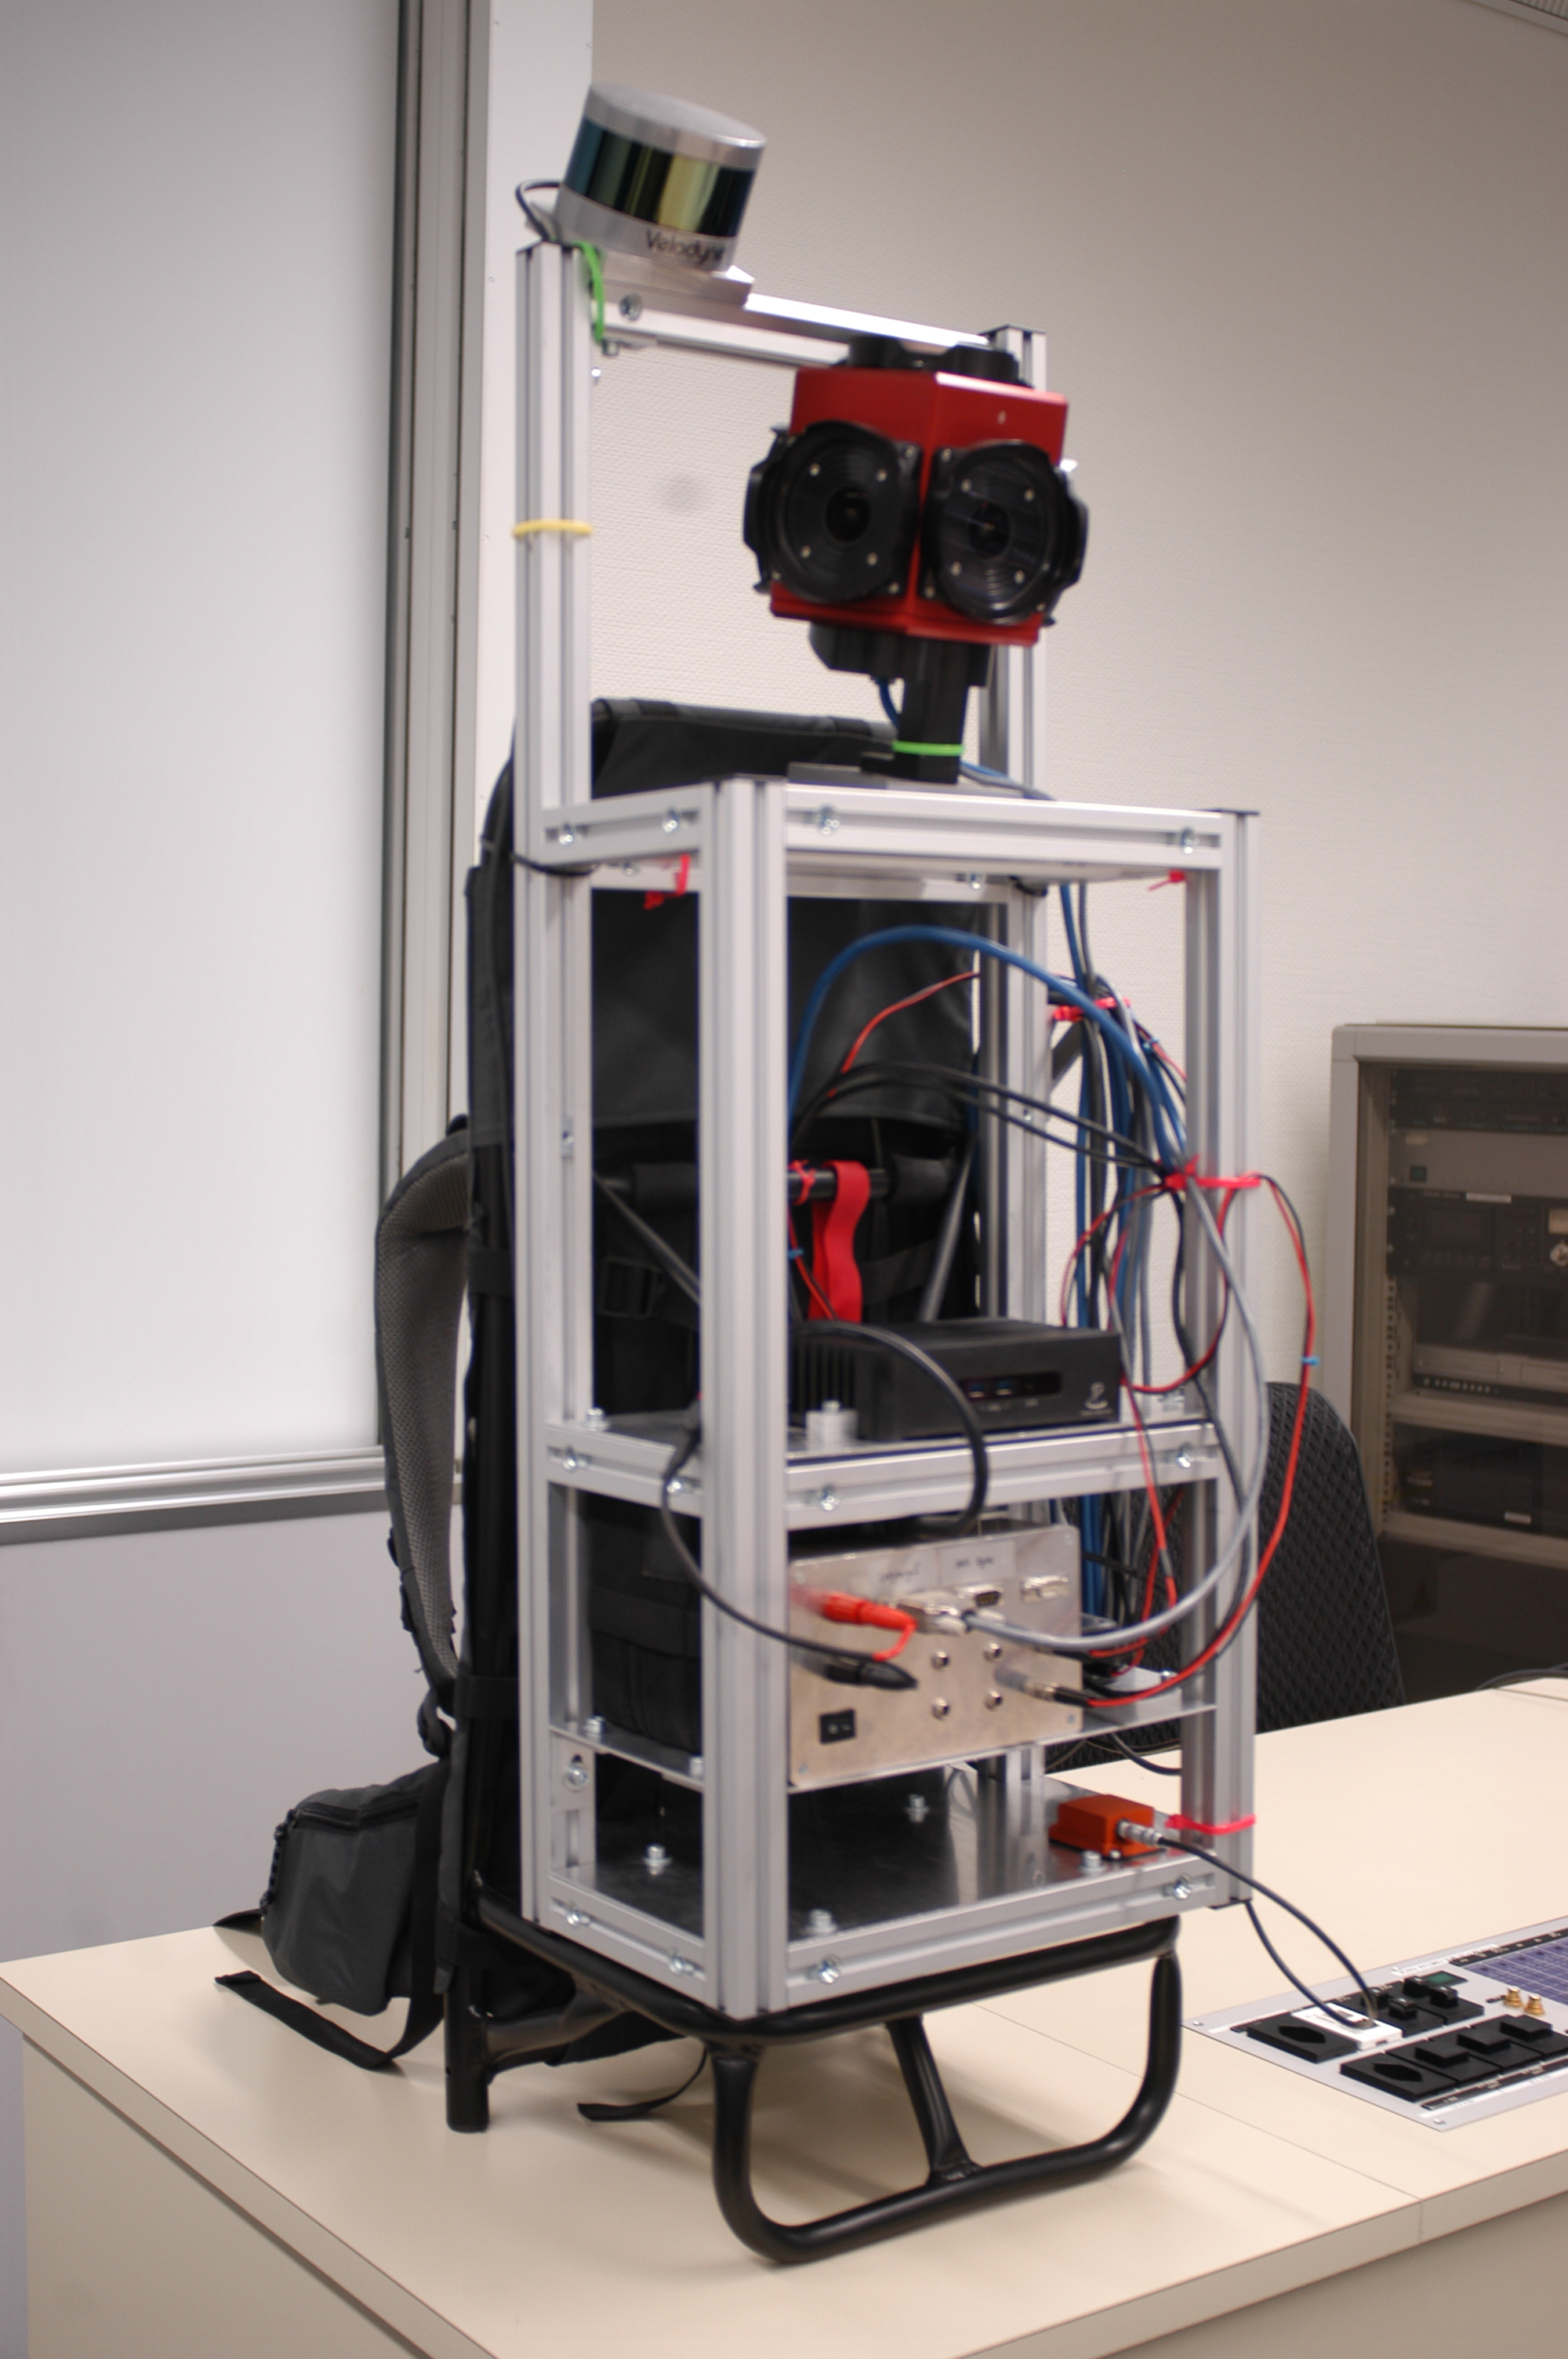
\includegraphics[height=0.7\textheight]{./Abbildungen/cappro_3.JPG}
    \end{column}
    \begin{column}{0.66\textwidth}
      \begin{tabular}{ll}
 	\multicolumn{2}{l}{Integrierte Sensoren:}\\
	\textbf{Kamera} & Ladybug5\\
	\textbf{Laserscanner} & Velodyne VLP-16\\
	\textbf{IMU} & XSens MTI-200\\
	&\\
 	\multicolumn{2}{l}{Software (Open-Source):}\\
	
\includegraphics[height=0.5cm]{./Abbildungen/ros_logo.png} & Robot Operating System (ROS) \\
	
\includegraphics[height=0.7cm]{./Abbildungen/20636162.png} & Google Cartographer (SLAM)\\
	
\includegraphics[height=0.7cm]{./Abbildungen/opengraph-icon-200x200.png} & Python\\
	
\includegraphics[height=0.7cm]{./Abbildungen/cpp_logo.png} & C++
       \end{tabular}
    \end{column}
  \end{columns}
  \end{frame}

% - evtl. Kurzvideo Betrieb
\begin{frame}[plain]
  \begin{tikzpicture}[remember picture,overlay]
    \node[anchor=south west, inner sep=0pt] at (current page.south west) {
    \movie[showcontrols]{\includegraphics[width=1\paperwidth]{./Abbildungen/CaptureProBackpack.JPG}}{./Abbildungen/cappro_opt.mp4}
    };
  \end{tikzpicture}
\end{frame}

% Ausblick
\begin{frame}
\frametitle{Fazit \& Ausblick}
  \begin{itemize}
   \item Fazit
   \begin{itemize}
    \item Indoor Mobile Mapping-System entwickelt
    \item Endergebnisse: Orientierte Bilder (Näherungswerte)
    \pause
    \item Forschungsprototyp $\rightarrow$ Untersuchung verschiedener Sensorkonfigurationen (Positionierung und Datenerfassung)
    \pause
    \item Online-SLAM
   \end{itemize}
   \pause
   \item Ausblick
   \begin{itemize}
    \item Beleuchtung / Blitzlicht
    \pause
    \item $360^\circ$-Stereokonfiguration (orientierte 3D-Bilder)
    \pause
    \item Optimierung SLAM-Konfiguration
    \item Kalibrierung des Gesamtsystems
    \pause
    \item Indoor \& Outdoor-Navigation (zusätzliches GNSS\&INS)
   \end{itemize}
  \end{itemize}
\end{frame}

\begin{frame}
   \begin{columns}[onlytextwidth]
    \begin{column}{0.33\textwidth}
      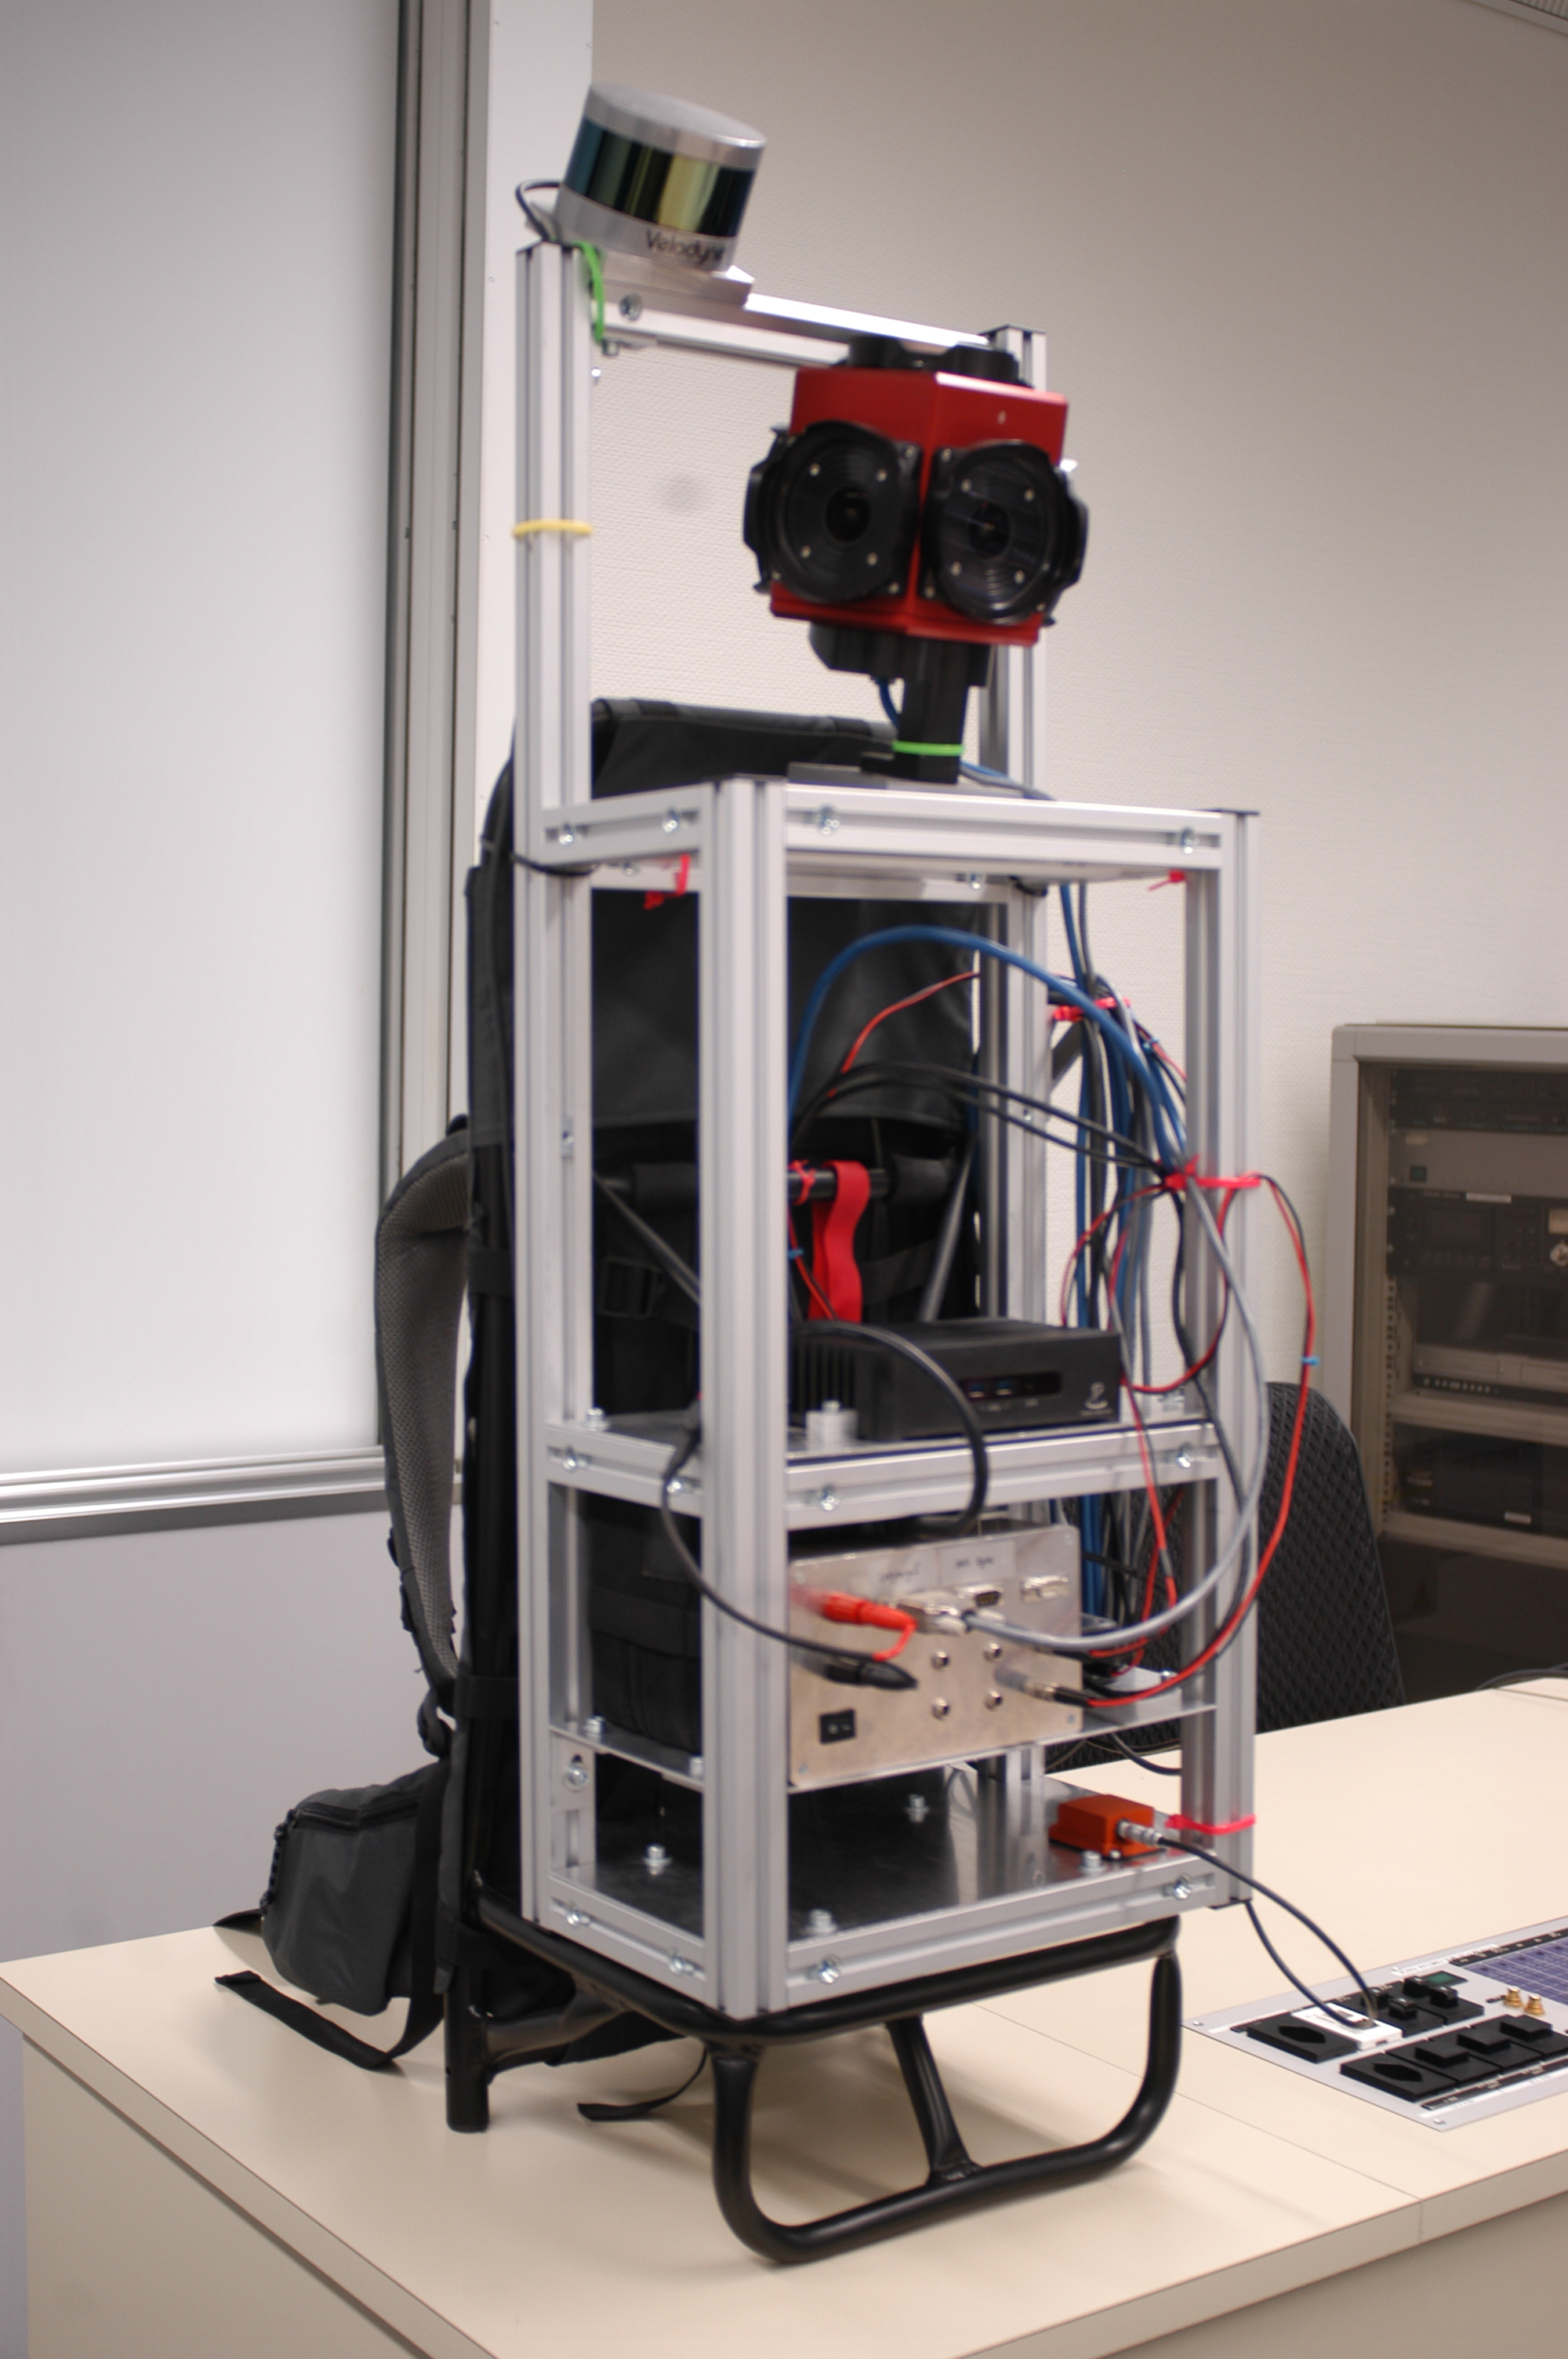
\includegraphics[height=0.7\textheight]{./Abbildungen/cappro_3.JPG}
    \end{column}
    \begin{column}{0.66\textwidth}
      \textbf{Besten Dank für Ihre Aufmerksamkeit!} \newline
      Fragen? \newline
      \newline
      Stefan Blaser\newline
      Wissenschaftlicher Mitarbeiter -- IVGI, FHNW\newline
      \href{mailto:stefan.blaser@fhnw.ch}{stefan.blaser@fhnw.ch}
    \end{column}
  \end{columns}
\end{frame}

\end{document}
